El perceptrón es un modelo de neurona artificial llamada unidad lógica de umbral (TLU, por sus siglas en inglés: Threshold Logic Unit) , desarrollado por Frank Rosenblatt en 1957. Es un modelo simple, donde una única neurona puede ser utilizada para problemas de clasificación binaria \cite{rosenblatt1957perceptron}.

El perceptrón es un caso particular y simple, con una función de activación específica y aplicable principalmente a problemas lineales. “En el caso del perceptrón, la elección de la función de activación de signo está motivada por el hecho de que es necesario predecir una etiqueta de clase binaria” \cite[p. 11]{aggarwal2018neural}. Esta función de activación suele ser una función escalón, produciendo una salida binaria (0 o 1).  Por lo tanto se utiliza para problemas de clasificación linealmente separables, lo que significa que solo puede resolver problemas donde se puede trazar una línea o un hiperplano para separar claramente las clases en un espacio de características.

\begin{figure}
	
	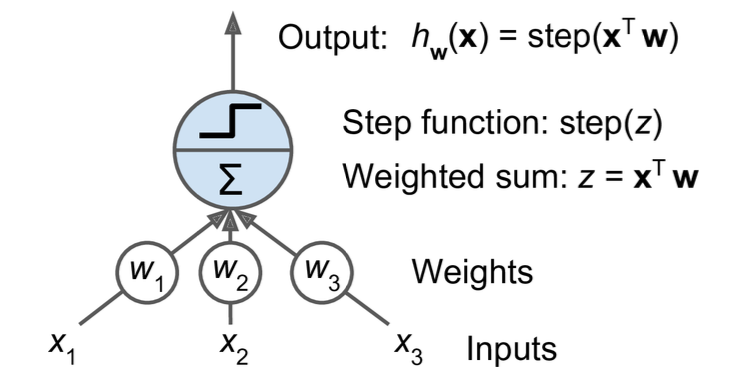
\includegraphics[width=0.65\textwidth]{capitulo2/figuras/an4.png}
	\caption{Unidad logica de umbral}
	\floatfoot{Fuente: Hands-on machine learning with Scikit-Learn, Keras, and TensorFlow \cite[p. 282]{geron2019hands}}
	\label{fig:an4}
\end{figure}

``El TLU calcula una combinación lineal de las entradas ( $\text{z} = w_1x_1 + w_2x_2 + \cdots + w_nx_n = x_Tw$) y si el resultado excede un umbral determinado en la función de paso , genera la clase positiva o genera la clase negativa''\cite[p. 282]{geron2019hands} ver Figura \ref{fig:an4}. 

La representación de una neurona artificial actual puede tener una función de activación más compleja que el escalón,  para permitir el aprendizaje en diferentes contextos. Por ejemplo, se puede emplear una función sigmoidal, tangente hiperbólica, ReLU, entre otras.






